\documentclass[12pt,a4paper]{article}
\usepackage[utf8]{inputenc}
\usepackage[french]{babel}
\usepackage[T1]{fontenc}
\usepackage{amsmath}
\usepackage{amsfonts}
\usepackage{amssymb}
\usepackage{graphicx}
\makeatletter
\@addtoreset{section}{part}
\@addtoreset{subsection}{part}
\@addtoreset{subsubsection}{part}
\makeatother
\title{Projet Méta-heuristiques (MPRO) : Couverture connexe minimum dans les réseaux de capteurs}
\author{Groleaz Lucas \\ Houdayer Antoine}

\begin{document}
\maketitle
\tableofcontents
\part{Sujet}
\section{Modélisation}
Dans tous le problème, on cherche à placer des capteurs sur une grille de façon optimale. Autrement dit, on peut placer des capteurs sur les points à coordonnées entières qui sont à l'intérieur d'une zone prédéfinie. Dans toute la suite on travaillera sur des grilles carrées, pour alléger les notations. On notera $n$ la dimension de la grille. Ainsi chaque sommet $v$ de la grille est un élément de $V=[\![1,n]\!]\times [\![1,n]\!]$. On notera $S\subset V$ l'ensemble des sommets sur lesquels on a choisi de placer un capteur, c'est notre façon d'encoder la solution.

Chaque capteur est doté d'un rayon de captation $R_{capt}$, et d'un rayon de communication $R_{comm}\geq R_{capt}$.  On souhaite utiliser un minimum de capteurs tout en respectant deux contraintes.
\begin{itemize}
\item Contrainte de connexité : La grille est doté d'un puits, point de coordonnées $(1;1)$. Un capteur peut communiquer avec tout capteur ou avec le puits, à condition qu'il soit séparé de ce dernier d'une distance inférieure ou égale à $R_{comm}$. Tout capteur doit pouvoir communiquer avec le puits, soit directement, soit par l'intermédiaire d'autres capteurs. 

\item Contrainte de couverture : Tout sommet de la grille, excepté le puits, doit être à une distance inférieure ou égale à $R_{capt}$ du capteur le plus proche.

\end{itemize}

\begin{figure}[h]
\begin{center}
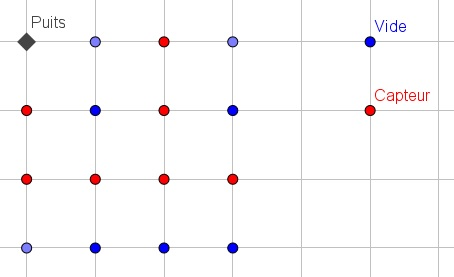
\includegraphics[scale=1]{Images/4_1_1_realisable.jpg}
\caption{Exemple de solution réalisable pour $n=4$, $R_{capt}=R_{comm}=1$, ici $|S|=7$}
\end{center}
\end{figure}

N.B: Il n'est pas interdit de couvrir le puits (ce qui est même inévitable si $R_{capt}=R_{comm}$), ou d'y placer un capteur, mais l'expérience montre qu'il n'est pas intéressant en pratique de placer un capteur dans un coin de la grille. Comme le puits est un point particulier, on doit appliquer un traitement particulier aux capteurs que l'on place dessus.
 Notamment, si on enlève un capteur situé sur le puits, les autres capteurs continuent de communiquer avec le puits. De plus avec les nombreuses rotations et symétries possibles, il faudrait que toutes les solutions optimales aient des capteurs aux quatre coins pour qu'interdire un capteur sur le puits soit impactant. Ainsi, nous avons pris le parti de ne pas mettre de capteur sur le puits. Bien sûr, il faut toujours envisager cette option dans les parties théoriques. 

\section{Reformulation}
Nous avons adopté une reformulation du problème à base de graphes, un pour chaque contrainte. On note $p=(1;1)$, le puits. 
Pour une solution $S$ donnée, non nécessairement réalisable, on défini les ensembles d'arêtes $E_{capt}(S)$, l'ensemble des liens de captations, et $E_{comm}(S)$ l'ensemble des liens de communication. Formellement on a :
\[E_{capt}(S)=\{\{v_1,v_2\}|v_1\in V,\,v_2\in S\setminus v_1,\, \Delta(v_1,v_2)\leq R_{capt}\}\] 
\[E_{comm}(S)=\{\{v_1,v_2\}|v_1,\,v_2\in S\cup \{p\},\ v_1\neq v_2,\,\Delta(v_1,v_2)\leq R_{comm}\}\] 
On peut alors construire les graphes correspondants:
\[G_{capt}(S)=(V,E_{capt}(S))\]
\[G_{comm}(S)=(S\cup p,E_{comm}(S))\]
Ci-dessous, une illustration dans le cas $n=4$, $R_{capt}=1$, $R_{comm}=2$. On a laissé tous les sommets de $S$ sur le schéma pour plus de lisibilité.
\begin{figure}[!h]
\center
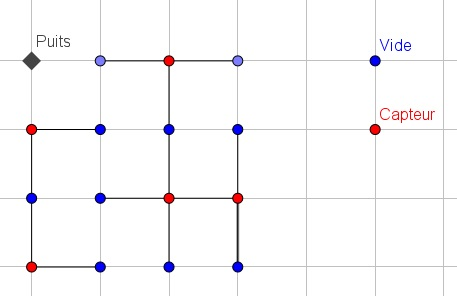
\includegraphics[scale=1]{Images/4_1_2_captgraph.jpg}
\caption{Graphe de captation $G_{capt}(S)$}
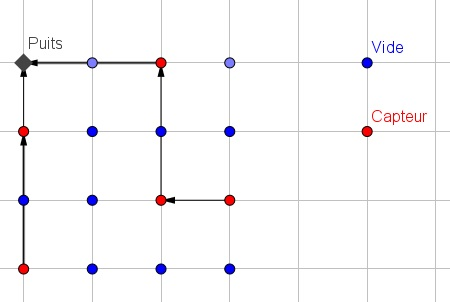
\includegraphics[scale=1]{Images/4_1_2_commgraph.jpg}
\caption{Graphe de communication $G_{comm}(S)$}
\end{figure}
\\N.B. : Sur le graphe de $G_{comm}$, on a représenté les arrêtes par des flèches, pour illustrer la notion de puits. Cependant, le graphe n'est pas intrinsèquement orienté, et il pourrait tout à fait présenter des cycles.

Le problème peut alors se reformuler de la façon suivante :
\begin{itemize}
\item Minimiser $|S|$.
\item Contrainte de connexité : $G_{comm}(S)$ est connexe.
\item Contrainte de couverture : $G_{capt}(S)$ n'a pas de sommet isolé autre que le puits.
\end{itemize}
\section{Détails d'implémentation}
Nous avons choisi d'utiliser le langage $C++$ pour tenter d'implémenter une méthode de résolution approchée du problème. Nous avons taché d'utiliser une implémentation du problème alliant simplicité d'utilisation et efficacité. Pour cela, nous utilisons un codage double des solutions:

Pour garder en mémoire quels sont les sommets sur lesquels un capteur est placé, le sommets captés, et les capteurs appartenant à la composant connexe du puits dans $G_{comm}(S)$, nous utilisons trois tableaux de bits de type bitset. Leurs principaux avantages sont leur faible occupation de mémoire, mais surtout la possibilité de les manipuler grâce à des opérations binaires. En contrepartie, leur taille doit être fixée à la compilation. Nous les avons déclarés de taille $2500$, pour traiter des grilles ayant moins de $2500$ sommets. Nous aurions du utiliser des vector<bool> pour pouvoir traiter des problèmes de taille arbitraire, mais en perdant la possibilité de faire des opérations binaires.

Nous gardons également en mémoire en permanence, les graphes $G_{comm}(S)$ et $G_{capt}(S)$, encodés comme étant pour chaque sommet, une liste de ses voisins dans le graphe, c'est-à-dire comme un tableau de listes de sommets. Pour être tout à fait rigoureux, plutôt que la structure "list" de la bibliothèque standard, nous avons créé une structure nommée GreedyList constituée d'un tableau pré-alloué associé à un compteur d'éléments. Ainsi, on évite les coûts de désallocation et allocation, principalement lors de la copie d'objets, économisant un temps non négligeable. Ces graphes sont tout à fait  adaptés à la structure du problème et permettent d'être performant lors du calcul d'un nouvel état obtenu par suppression ou ajout d'un capteur. Il suffit pour cela de précalculer les deux graphes suivants : 
\[G_{capt}=G_{capt}(V)\]
 le graphe de tous les liens de captation possibles, et
\[G_{comm}=G_{comm}(V)\] 
le graphe de tous les liens de communication possibles. Un gros avantage de cette méthode est que l'on s'affranchit en partie de la définition initiale du problème. Pour peu que l'on puisse calculer les graphes $G_{comm}$ et $G_{capt}$, on peut facilement adapter le programme pour travailler sur des grilles (finies) de forme arbitraire, une disposition des points arbitraire, des calculs de distance différents, comme une portée différente suivant la position du capteur etc...

D'un point de vue plus pratique, sont codées les fonctions d'ajout et de suppression de capteur, qui gèrent l'utilisation et l'intégrité des objets mentionnés ci-dessus. On est alors libre d'utiliser ces fonctions et les dits objets pour travailler sur le problème. Notons que la fonction de suppression de capteur est relativement gourmande en calcul, puisqu'elle effectue un parcours en profondeur du graphe $G_{comm}(S)$ pour déterminer quelle est la nouvelle composante connexe du puits.



Nous avons alors essayé deux approches du problème très différentes.

\part{Approche par chaînes d'exclusion}
Dans toute cette partie, on illustrera les méthodes présentées sur l'instance $(P)$ du problème : $n=4$, $R_{capt}=R_{comm}=1$.
\section{Heuristique}
\subsection {Heuristique déterministe}
Dans cette approche, on construit tout simplement une solution $S$ en positionnant des capteurs sur la totalité de la grille, pour avoir une solution réalisable. On tente alors de retirer les capteurs un à un lorsque c'est possible sans compromettre la réalisabilité de la solution.
Illustrons la méthode sur $(P)$ (voir figure): 
\begin{figure}[h]
\center
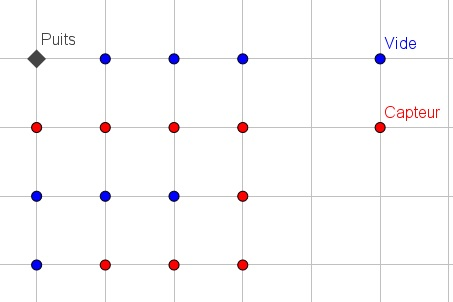
\includegraphics[scale=1]{Images/4_1_1_naif.jpg}
\caption{Résultat de l'heuristique d'exclusion sur $(P)$}
\end{figure}

Procédons dans l'ordre, ligne par ligne :  on peut enlever la première ligne sans problème, cependant, on doit alors conserver $(2;1)$ pour ne pas déconnecter le reste des capteurs. On doit également garder le reste de la seconde ligne pour continuer à capter la première. On peut alors retirer la troisième ligne, à l'exception de $(3;4)$ qui est alors nécessaire pour connecter la dernière ligne. On peut ensuite enlever $(4,1)$. On constate qu'on est alors obligés de garder le reste de la dernière ligne.

Si l'on note les sommets par leur indice $k=n(i-1)+(j-1)$ plutôt que par leurs coordonnées $(i;j)$, pour plus de concision, on obtient
\[S=\{4,5,6,7,11,13,14,15\}\]

À première vue, cette heuristique présente de quelques défauts, et assez peu de qualités. Tout d'abord cette heuristique est chronophage : on essaye de retirer un à un les capteurs (initialement au nombre de $n^2$), ce qui implique d'effectuer un parcours en profondeur des sommets restants pour vérifier la connexité. Le coût de construction d'une telle solution est donc de $O(n^4)$. Deuxièmement, la structure induite par une telle construction est peu désirable en pratique, on obtient en général des solutions de qualité médiocre. Elle a toutefois l'avantage d'être implémentée en seulement quatre lignes de code. Elle a également l'avantage de garantir que la solution obtenue est réalisable. 
\subsection{Heuristique aléatoire} 
On peut apporter à cette heuristique une très simple amélioration ,visant à briser la structure induite par la méthode déterministe. Pour cela, il suffit de remarquer que la solution obtenue est très dépendante de l'ordre dans lequel on a essayé de retirer les sommets (ligne par ligne dans l'exemple). On choisit alors au hasard un ordre dans lequel on va retirer les capteurs, c'est-à-dire une permutation des sommets. Par exemple si on tire au hasard la permutation suivante : \[0,10,11,12,13,5,8,15,9,6,4,3,14,1,2,7\] on obtiendra le résultat représenté sur la figure ci-dessous.
\begin{figure}[h]
\center
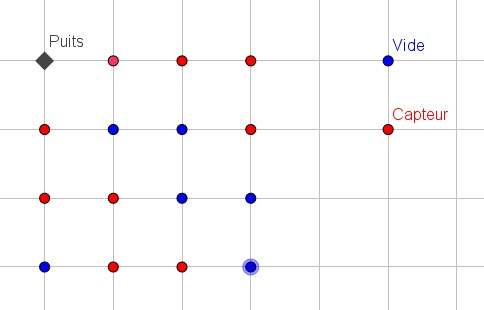
\includegraphics[scale=1]{Images/4_1_1_random.jpg}
\caption{Résultat pour une permutation au hasard}
\end{figure}

Bien sûr, cela ne garantit pas l'obtention d'une meilleur solution mais donne effectivement des solutions meilleures en moyenne que celles de l'heuristique déterministe, pour une instance quelconque. En annexe est fourni un jeu de résultats obtenus sur les instances de test.


\section{Les chaînes d'exclusion}
\subsection{Définition}
Dans notre problème, $S$ représente un ensemble de sommets. Au début de la méthode, $S$ comprend la totalité des sommets disponibles, puis on essaye un à un de les exclure de $S$. Voyons comment cette méthode peut être étendue formellement à une classe de problèmes plus large.

\subsubsection{Définition générale}
Soit $(P)$ un problème d'optimisation réalisable (dont l'ensemble des solutions réalisables est non vide), dont chaque solution réalisable ou non peut être encodée par un ensemble $S\subset \Sigma \;\text{fini}$, et dont tout $S\subset \Sigma$ encode une solution. On peut donc confondre solutions et sous-ensembles de $\Sigma$. On exige également que $(P)$  vérifie la propriété de transitivité suivante :
\[\forall S,S'\subset \Sigma,S\subset S',S \;\text{réalisable} \Rightarrow  S'\;\text{réalisable}\]
ou de façon équivalente
\[\forall v \in \Sigma\setminus S, S \text{ réalisable} \Rightarrow S\cup v \text{ réalisable} \]
Autrement dit , en ajoutant un élément à une solution réalisable, on obtient une solution elle aussi réalisable. Comme $(P)$ est réalisable, on déduit de la propriété de transitivité que $\Sigma$ est réalisable. On défini alors l'ensemble des chaînes d'exclusion $L$ comme étant l'ensemble des permutations de $\Sigma$ (on rappelle que $\Sigma$ est fini). Pour tout $l\in L$, pour tout $k\in[\![1;|\Sigma |]\!]$, $l(k)$ est alors un élément de $\Sigma$.

Pour tout $l\in L$, on défini alors la solution engendrée par $l$, notée $S(l)$. $S(l)$ est construit récursivement, à partir de la solution $S_0(l)=\Sigma$ suivant la relation de récurrence suivante : $S_{k}(l)=S_{k-1}(l)\setminus l(k)$ si $S_{k-1}(l)\setminus l(k)$ est une solution réalisable, et $S_{k}(l)=S_{k-1}(l)$ sinon, pour tout $k\in[\![1;|\Sigma |]\!]$. On prend alors $S(l)=S_{|\Sigma |}(l)$, le dernier élément de la suite. Par construction, $S(l)$ est donc réalisable pour tout $l\in L$. Nous verrons ci-après deux propriétés des chaînes d'exclusion, et pourquoi la propriété de transitivité est cruciale.  

N.B.:Il est tout à fait possible de transposer cette définition pour un problème vérifiant la propriété de transitivité inverse, pour un problème dans lequel on part de $S_0=\emptyset$ auquel on essaye d'inclure des éléments, comme par exemple pour le problème de sac à dos.

\subsubsection{Dans le problème de couverture connexe dans un réseau de capteurs}
Dans notre problème, $\Sigma$ est l'ensemble $V$ des sommets. $S\subset \Sigma$ représente l'ensemble des sommets sur lesquels un capteur est placé, on a donc bien équivalence solution / sous-ensemble de sommets. Démontrons alors que la propriété de transitivité est vérifiée.
\paragraph{Démonstration}
Si $\Sigma$ est la seule solution réalisable, la transitivité est triviale. Sinon, soit $S\neq \Sigma$ une solution réalisable. Soit $v \in V$ tel que $v\notin   S$. Montrons que $S'=S\cup v$ est réalisable. On doit montrer que les contraintes de couverture et de connexité de $S'$ sont vérifiées.

Trivialement, la contrainte de couverture est toujours vérifiée. En effet, ajouter un capteur à $S$ a pour effet d'ajouter des arêtes dans $G_{capt}(S)$. Ainsi $G_{capt}(S)\subset G_{capt}(S')$. Le graphe n'ayant aucun point isolé sauf le puits avant ajout d'arêtes vérifiera toujours la propriété après ajout. 

Montrons maintenant que $G_{comm}(S')$ est connexe. Il suffit pour cela que $v$ puisse se connecter à $G_{comm}(S)$, i.e. qu'il existe une arrête dans $G_{comm}$ entre $v$ et un sommet de $S$. Comme la propriété de couverture est respectée pour $S$, il existe une arrête dans $G_{capt}$ entre $v$ et un sommet de $S$. Or, $R_{capt}\leq R_{comm}$, ce qui implique $G_{capt}\subset G_{comm}$. Autrement dit, à chaque lien possible de captation correspond un lien de communication. Un nouveau capteur $v$ pourra donc se connecter par le même lien qui lui permettait d'être capté avant l'ajout du capteur.

On a bien montré que notre problème vérifiait la propriété de transitivité, et qu'il appartient donc bien à la classe de problème définie plus haut.

\subsection{Propriétés}
\subsubsection{Chaînes d'exclusion et solutions non dégénérées}

On reprend dans cette partie la classe de problèmes plus générale, avec les notations alors introduites.

 \paragraph{Solution dégénérée}
 
On dit qu'une solution réalisable $S$ est dégénérée si il existe $S'\subset S$ tel que $S'$ soit réalisable ; ou de façon équivalent grâce la propriété de transitivité ; si il existe $v\in S$ tel que $S\setminus v$ soit réalisable.

On a alors le lemme suivant :
\[\forall l\in L,\; S(l)\;\text{est non dégénérée}\]

Démonstration par l'absurde : 
\\Soit $l$ une chaîne d'exclusion telle que $S(l)$ soit dégénérée. 
\\Soit $v\in S(l)$ tel que $S(l)\setminus v$ soit réalisable.
\\Soit $k$ tel que $l(k)=v$.
Nécessairement puisque $v\in S(l)$, $S_{k-1}(l)\setminus v$ n'est pas réalisable. Or par construction $S(l)\subset S_{k-1}(l)$ et donc a fortiori $S(l)\setminus v \subset S_{k-1}(l)\setminus v$. La propriété de transitivité n'est donc pas respectée.
On en déduit alors bien que $S(l)$ est nécessairement non dégénérée.

\paragraph{Construction d'une chaîne d'exclusion génératrice}
Soit $S$ une solution quelconque, réalisable ou non. On définit alors $l^c$ comme étant la liste dans un ordre arbitraire des  $v\in \Sigma$ pour lesquels $v\in S$. De même on définit $l^e$ comme étant la liste dans un ordre arbitraire des $v\in \Sigma$ pour lesquels $v\notin S$. On note $l^e+l^c$ la concaténation de ces deux listes (avec $l^e$ en premier). Par définition $l^e+l^c$ contient une et une seule fois tous les éléments de $\Sigma$, et est donc bien une chaîne d'exclusion. On observe alors la propriété suivante:

\[S=S(l^e+l^c) \Leftrightarrow S\;\text{est non dégénérée}\]


Démonstration :

Le sens direct est une conséquence immédiate du lemme. En effet il énonce que $S(l^e+l^c)$ est non dégénérée. Il faut donc montrer le sens indirect.

Expliquons d'abord l'essence de cette implication. On souhaite montrer que si on dispose d'une solution non dégénérée $S$, on est capable de construire une chaîne d'exclusion qui l'engendre. Le raisonnement est le suivant : je part de $S_0=\Sigma$, et je souhaite exclure des éléments de $\Sigma$ un à un pour aboutir à $S$, en passant uniquement par des solutions réalisables. Il va de soi que si j'arrive à enlever tous les éléments de $l^e$, j'aurais atteint $S$, et je ne pourrais enlever aucun élément de $l^c$ puisque $S$ est non dégénérée. Il suffit donc de montrer que quel que soit l'ordre dans lequel j'essaie d'enlever les éléments de $l^e$, je ne passerais que par des solutions réalisables. Nous allons pour cela démontrer le cheminement inverse :  si je part de $S$ et que j'ajoute les capteurs manquants dans un ordre arbitraire, je ne passerais que par des solutions réalisables. Récursivement, il suffit donc de montrer qu'en ajoutant un capteur à une solution réalisable, j'obtiens encore une solution réalisable. Il s'agit de la propriété de transitivité. La propriété de construction est donc démontrée.

On peut déduire de la propriété de construction la propriété plus faible de caractérisation d'une solution non dégénérée suivante
\[S\text{ non dégénérée} \Leftrightarrow \exists l\in L, S(l)=S\]

On a donc démontré que pour chaque solution non dégénérée on pouvait construire facilement une chaîne d'exclusion qui la génère, et donc qu'il en existe une. On peut donc en toute légitimité encoder un solution non dégénérée par une de ses chaînes d'exclusion. Supposons maintenant que le retrait d'éléments dans $S$ améliore toujours la fonction objectif (dans un sens ou dans l'autre suivant si l'on maximise ou minimise), les solutions optimales sont alors non dégénérées et les solution non dégénérées sont en un sens des optimums locaux. Moralement on démontre que les chaînes d'exclusion sont adaptés pour résoudre un problème qui vérifierait cela, tel que le problème de couverture connexe minimum.  


Remarque : Je notais précédemment que notre implémentation du problème de couverture connexe permettait de traiter des variantes avec d'autres définitions de distance. On voit ici que la propriété de construction (et les méthodes qui en découlent) n'est vraie que si la propriété de transitivité est vraie. Or on l'a vu, cette propriété découle de $G_{capt}\subset G_{comm}$. En particulier, il serait impossible de travailler avec cette méthode si on avait $R_{comm}<R_{capt}$.

\subsubsection{Chaînes équivalentes}
On retourne désormais sur le problème de couverture connexe minimale.
\\Lorsqu'on code une solution quelconque, pas forcément réalisable, avec son vecteur binaire, il découle immédiatement que pour une grille de dimension $n$, il existe $2^{n^2}$ solutions possibles. De plus, seulement une partie infime de ces solutions, les solutions non dégénérées, peut être associée à une chaîne d'exclusion.

Or, une chaîne d'exclusion étant essentiellement une permutation, il existe $n^2!\gg 2^{n^2}$ chaînes d'exclusion. On en déduit qu'il existe probablement pour chaque chaîne d'exclusion un nombre colossal de chaînes d'exclusion équivalentes, c'est-à-dire engendrant la même solution.

En particulier, on a vu que toute chaîne d'exclusion engendre une solution non dégénérée, et que de cette solution on peut reconstruire une chaîne l'engendrant, en utilisant la partition $S$ et $V\setminus S$ , l'ordre étant sans importance.


\section{Voisinage induit}
\subsection{Définition et propriétés}
Lorsque qu'on cherche une structure de voisinage, on cherche une façon qui fait sens de modifier légèrement le vecteur qui encode la solution. Par exemple dans le problème du sac à dos, on peut essayer d'ajouter un objet dans le sac, quitte à appliquer après une heuristique de réparation. Dans notre problème on souhaiterait par exemple déplacer légèrement un capteur, ou en supprimer quelques uns. Il n'est cependant pas facile de faire une heuristique de réparation assez efficace pour avoir une meilleure solution après.

C'est là qu'est la force des chaînes d'exclusion : en appliquant une légère modification à une chaîne d'exclusion et en l'appliquant, on obtient une solution S légèrement modifiée, réalisable mais surtout non dégénérée! Autrement dit, en un sens, on peut facilement créer un voisinage dans lequel toutes les solutions sont "de qualité".

Le voisinage utilisé par la suite est le suivant :
Soit $S$ une solution. On construit les suites $l^e$ et $l^c$, puis on les mélange aléatoirement. On choisit au hasard un élément de $l^c$, qu'on retire de $l^c$ pour le mettre au début de $l^e$. On appelle $l'^e$ et $l'^c$ les suites ainsi obtenues. On construit alors une nouvelle solution $S'$ à partir de $l'=l'^e+l'^c$.
En faisant cela, on choisi en fait au hasard un capteur et on met son indice au début de la chaîne d'exclusion, on va donc faire en sorte  de ne pas mettre de capteur à cet endroit. La nouvelle chaîne $l'$ ne peut donc pas générer $S$. Au vu de la quantité de permutations équivalentes, cela aurait pu être un risque.

Remarques:

Sans que ce soit gênant, on peut noter que $S$ n'est pas nécessairement dans le voisinage de $S'$.

Par ailleurs, toujours sans que ce soit gênant,si $S$ est dégénérée, il se peut que $S(l)$ avec $l=l^e+l^c$ ne soit pas "proche" de $S$. Il va alors de soit que $S'$ n'est pas nécessairement "proche" de $S$.

Dans toute la suite on travaillera de toute façon uniquement sur des solutions non dégénérées. 
\subsection{Exemple}
Soit la solution non dégénérée obtenue avec l'heuristique déterministe.
On rappelle qu'on avait alors
\[l=(0,1,2,3,4,5,6,7,8,9,10,11,12,13,14,15)\] 
\[S(l)=\{4,5,6,7,11,13,14,15\}\]
\begin{figure}[h]
\center
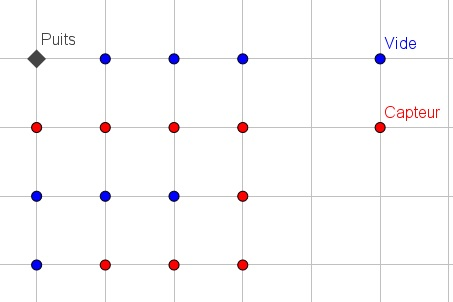
\includegraphics[scale=1]{Images/4_1_1_naif.jpg}
\caption{Résultat de l'heuristique d'exclusion sur $(P)$}
\end{figure}

On construit donc 
\[l^e=(0,1,2,3,8,9,10,12)\]
\[l^c=(4,5,6,7,11,13,14,15)\]
On mélange aléatoirement
\[l^e=(8,0,9,10,3,1,12,2)\]
\[l^c=(13,7,5,6,15,11,14,4)\]
On prend un sommet de $l^c$ qu'on met au début de $l^e$, par exemple $15$, on impose alors de ne pas mettre de capteur dans le coin inférieur droit.
\[l'^e=(15,8,0,9,10,3,1,12,2)\]
\[l'^c=(13,7,5,6,11,14,4,12)\]
On obtient alors 
\[l'=(15,8,0,9,10,3,1,12,2,13,7,5,6,11,14,4)\]
A première vue, il pourrait sembler que cette chaîne d'exclusion est très différente de la chaîne ordonnée, pourtant en appliquant la chaîne, on obtient
\[S'=\{4,5,6,7,10,13,14\}\]
Non seulement on est sur une solution très proche, mais elle utilise même un capteur en moins.
\begin{figure}[!h]
\center
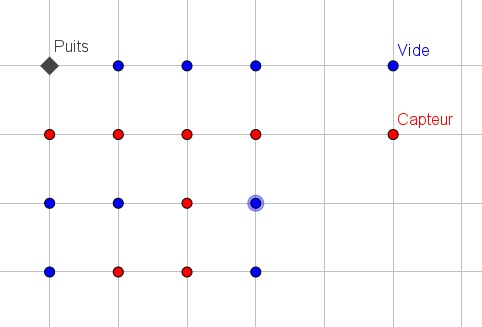
\includegraphics[scale=1]{Images/4_1_1_neigh.jpg}
\caption{Voisinage de la solution déterministe}
\end{figure}

Le principal défaut réside dans le temps de calcul nécessaire pour générer une solution avec une chaîne d'exclusion. Même si le problème est simple, la complexité est au moins de l'ordre de la longueur du vecteur binaire sur lequel on travaille, ici $n^2$. A cause du parcours en profondeur dans ce problème en particulier on est même en $O(n^4)$.  

Remarques : La taille du voisinage est démesurée, il est déconseillé d'appliquer des technique de parcours méthodique telles que la recherche de voisinages améliorants, ou la recherche avec tabous. Dans la section suivante, on l'utilise dans l'algorithme du recuit simulé.
\section{Recuit simulé}
Pour obtenir une solution approchée de qualité, nous avons utilisé ce voisinage avec la méta-heuristique de recuit simulé. Le nombre d'itérations par palier de température à été choisi proportionnel au nombre de capteurs utilisés. Le problème de notre voisinage étant déjà la vitesse on a pris $0.85$ comme paramètre de décroissance de la température. La différence entre une solution et celles de son voisinages étant typiquement de l'ordre de l'unité, l'expérience confirme qu'il est inutile de commencer avec une température initiale supérieure à $1$. Les principaux réglages sont donc, le coefficient de proportionnalité $K$ entre le nombre de capteurs et le nombre d'itérations, ainsi que les critères d'arrêt.

Concernant les critères d'arrêt, on impose de descendre à une température inférieure à $0.1$. On s'arrête alors lorsqu'on ne parvient pas à améliorer le résultat pendant deux paliers de température consécutifs.

En annexe des jeux de résultats pour $K=1.25$ et pour $K=5$.
\section{Optimisation}
\subsection{Principe}
On souhaite éviter de faire un parcours en profondeur total à chaque fois que l'on veut enlever un sommet. On pensera à vérifier d'abord si la contrainte de couverture est respectée, mais cela n'améliore pas vraiment en pratique car on doit au moins faire le parcours pour tous les capteurs qu'on enlève, c'est-à-dire beaucoup, d'autant plus si $R_{capt}$ est grand.

Une des caractéristique des chaînes d'exclusion est que l'on est jamais dans un état non réalisable. La seule question que l'on se pose est donc, étant donné un graphe connexe, y a-t-il un moyen de savoir facilement si le graphe est toujours connexe après retrait d'un sommet. 

Soit $k$ le sommet que l'on veut retirer. Il suffit de savoir si tous les voisins de $k$ (au sens de la communication) ont un chemin les reliant au puits n'utilisant pas $k$.

Pour cela on définit la fonction $\Delta$ par $\Delta (k)$ est la longueur du plus court chemin reliant $k$ au puits. Soit $k'$ un voisin de $k$. 

Si $\Delta(k')\leq \Delta(k)$, nécessairement il existe un chemin qui relie $k'$ au puits sans passer par $k$. Si $\Delta(k')=\Delta(k)+1$, mais qu'il existe un voisin $k''$ de $k'$ tel que $k''\neq k$ et $\Delta(k'')=\Delta(k)$, alors on peut rejoindre le puits depuis $k'$ par $k''$ plutôt que par $k$, sans que cela affecte la distance de $k'$ au puits. Si tous les voisins de $k$ vérifient une de ces deux propriétés, alors on peut supprimer $k$ sans compromettre la connexité, mais aussi sans changer la valeur de $\Delta$ pour les autres sommets. La suppression de $k$ est donc très peu coûteuse. 

Maintenant, supposons qu'un des voisins $k'$ de $k$ ne vérifie pas ces propriétés. Il y a alors deux cas de figure. Il est possible qu'il existe un chemin qui va relier $k'$ au puits, mais il faudra alors mettre à jour la distance de $k'$ mais aussi du reste du graphe (dans l'hypothèse bien sur qu'on supprime $k$ au final). Cela peut être fait en explorant seulement les sommets dont la valeur change, de façon intelligente. Il est également possible qu'on ne puisse pas relier $k'$ au puits, auquel cas on ne supprimera pas $k$.

Dans ces deux cas, il faut faire un parcours en profondeur en partant de $k'$ pour départager. On s'arrêtera dès qu'on rencontre un capteur différent de $k$ à même distance du puits que $k$. 

Dans les deux cas, lors du parcours en profondeur partant de $k'$ on peut stocker diverses informations quant à la forme du graphe. En particulier, on peut noter lorsqu'on rencontre une feuille, qui sera forcement amovible si on la rencontre plus tard (la couverture étant conservée bien sûr). On peut remarquer que si tous les voisins d'un sommet autre que celui d'où on vient sont des racines d'arbres, alors le sommet est inamovible. Il ne pourra pas devenir amovible par la suite comme on sait que toute chaîne d'exclusion génère une solution non dégénérée.

Résumons les différents cas de figure, dans l'ordre
\begin{itemize}
\item Si le sommet a été montré inamovible précédemment, on ne fait rien.
\item Si la contrainte de couverture est violée (rapide à vérifier), on ne fait rien.
\item Si la suppression du sommet n'affecte pas les distance, on peut le supprimer rapidement.
\item On effectue alors un parcours en profondeur : Si un des voisins du sommet ne peut pas se reconnecter (parcours en profondeur complet), on ne fait rien, mais on a acquis des informations utiles sur les parties du graphe qui sont des arbres.
\item Si on arrive à reconnecter tous les voisins (le parcours en profondeur est écourté), on a des informations utiles, on supprime $k$ et on met à jour les distances à moindre coût. 
\end{itemize}

En pratique si le rayon de communication est élevé on va tomber très souvent dans le 3ème cas. L'optimisation est donc plus efficace dans ces cas là, même si les voisinages (au sens de la communication) sont plus grand.

L'amélioration est substantielle, on va environ $7$ fois plus vite pour $R_{capt}=R_{comm}=1$, jusqu'à $15$ fois plus vite pour $R_{capt}= 3$ et $R_{comm}=4$.
\subsection{Exemple}
Illustrons cela par un exemple, dans lequel on représentera chaque sommet par sa distance au puits ($\infty$ si il n'y a pas de capteur). On ajoutera un $i$ en indice si on a montré qu'un sommet est inamovible.
On considère qu'il n'y a pas de capteur sur le puits. La grille initial est la suivante
\begin{center}
\begin{tabular}{|c|c|c|c|}
\hline 
0 & 1 & 2 & 3 \\ 
\hline 
1 & 2 & 3 & 4 \\ 
\hline 
2 & 3 & 4 & 5 \\ 
\hline 
3 & 4 & 5 & 6 \\ 
\hline 
\end{tabular}
\end{center}

Considérons le capteur d'indice $9$, c'est-à-dire le capteur $(3;2)$. Il est situé à distance $3$ du puits. Il a deux voisins à distance $2$ qui ne posent pas problème, et deux voisins à distance $4$ mais qui ont tous deux un autre voisin à distance $3$. On peut donc supprimer le capteur d'indice $9$ sans faire de calculs coûteux, et aucune distance n'est modifiée. On obtient la grille suivante.

\begin{center}
\begin{tabular}{|c|c|c|c|}
\hline 
0 & 1 & 2 & 3 \\ 
\hline 
1 & 2 & 3 & 4 \\ 
\hline 
2 & $\infty$ & 4 & 5 \\ 
\hline 
3 & 4 & 5 & 6 \\ 
\hline 
\end{tabular} 

\end{center}
Essayons maintenant de supprimer le capteur d'indice $1$, le capteur $(1;2)$. On remarque que le capteur situé à sa droite n'a aucun autre voisin à distance $1$ que le capteur qu'on veut enlever. Cependant un rapide parcours en profondeur révèle qu'il peut toujours rejoindre le puits par un autre chemin, on peut le supprimer et mettre à jour les distances.

\begin{center}
\begin{tabular}{|c|c|c|c|}
\hline 
0 & $\infty$ & 4 & 5 \\ 
\hline 
1 & 2 & 3 & 4 \\ 
\hline 
2 & $\infty$ & 4 & 5 \\ 
\hline 
3 & 4 & 5 & 6 \\ 
\hline 

\end{tabular} 
\end{center}

On peut maintenant sans affecter les distance supprimer le capteur d'indice $2$. On a alors

\begin{center}
\begin{tabular}{|c|c|c|c|}
\hline 
0 & $\infty$ & $\infty$ & 5 \\ 
\hline 
1 & 2 & 3 & 4 \\ 
\hline 
2 & $\infty$ & 4 & 5 \\ 
\hline 
3 & 4 & 5 & 6 \\ 
\hline 

\end{tabular} 
\end{center}

Essayons maintenant de supprimer le capteur d'indice $4$, au sud du puits. Le parcours en profondeur révèle qu'on ne peut pas le supprimer. Cependant, on a par la même occasion remarqué que le capteur d'indice $3$ étant une feuille, son voisin, le capteur d'indice $7$ ,est inamovible. La configuration est donc la suivante.

\begin{center}
\begin{tabular}{|c|c|c|c|}
\hline 
0 & $\infty$ & $\infty$ & 5 \\ 
\hline 
$1_i$ & 2 & 3 & $4_i$ \\ 
\hline 
2 & $\infty$ & 4 & 5 \\ 
\hline 
3 & 4 & 5 & 6 \\ 
\hline 

\end{tabular} 
\end{center}

Ne ne ferons pas l'exemple en entier mais si ici on voulait enlever le capteur d'indice $5$, on se rendrait compte que c'est impossible car il faut couvrir $1$ (il n'y a pas de capteur sur le puits), sans faire quelque parcours.
\section{Parallélisation}
Nous avons essayé de paralléliser l'algorithme de recuit simulé. Chaque thread calcul alors un voisinage de la solution en cours. La principale question est donc de savoir sous quelle condition faire changer la solution en cours. 

La solution la plus simple est que chaque thread travaille indépendamment sur sa propre solution en cours, i.e. chaque thread effectue un recuit simulé et on conserve la meilleure solution à la fin. Cependant on voit dans l'annexe que l'écart type des solutions d'un recuit simulé est d'environ $2$, de façon peu dépendante du temps de calcul. Il est donc à prévoir et on vérifie par l'expérience que cette implémentation n'apporte qu'une amélioration de $3-4$ en moyenne pour un même $K$.

La deuxième solution relativement simple est de laisser chaque thread évoluer indépendamment jusqu'à l'obtention d'une solution améliorante, on synchronise alors chaque thread sur cette solution. Nous avons obtenu des résultats satisfaisants avec cette technique. Cependant à cause de la même remarque que pour la technique précédente, on peut penser que l'efficacité des threads en recherche indépendante est limitée.

La troisième solution est de laisser les threads chercher indépendamment jusqu'à ce que l'un d'entre eux trouve une solution qu'il veut accepter (pas forcément améliorante). On interromps alors le calcul des autres threads pour les synchroniser avec cette nouvelle solution. Cependant il n'est pas possible en pratique d'imposer tant de synchronisation entre les threads, on leur laisse alors finir leurs calculs et ils se synchroniseront d'eux-mêmes si la solution en cours a changée depuis le dernier passage (grâce à un système de flags), abandonnant alors le calcul qu'ils ont fait. Bien sûr, une solution améliorante est toujours conservée en priorité sur les autres.
\\Au premier abord il semblerait que beaucoup de temps de calcul est gaspillé avec cette technique mais elle obtient les meilleurs résultats en pratique (voir annexe). On peut peut-être interpréter cela comme étant le  résultat d'un meilleure synergie entre les threads, comme ils cherchent dans une direction plus commune, la recherche est plus organisée en somme.

N.B: Les tests ont été effectués sous les même conditions d'arrêts et de température que les tests sans parallélisation. Seul le coefficient de proportionnalité entre nombre de capteurs et nombre d'itérations par palier $K$ varie. 
\part{Annexe}
Tous les résultats sont donnés en nombre de capteurs, en colonne $n$ et les paires $(R_{capt};R_{comm})$ sur les lignes.

Ci-dessous les bornes inférieures calculées à partir des surface en nombres de point couvertes par un capteur. Si les rayons de communication et de captation sont égaux, on prend en compte que les rayons vont forcément se chevaucher d'une case. Ces bornes sont de mauvaise qualité mais on peut difficilement faire mieux.

\begin{center}
\begin{tabular}{|c|c|c|c|c|c|c|c|}
\hline
&10 & 15 & 20 & 25 & 30 & 40 & 50\\
\hline 
(1;1) & 25 & 56 & 100 & 156 & 225 & 400 & 625 \\ 
\hline 
(1;2) & 20 & 45 & 80 & 125 & 180 & 320 & 500 \\ 
\hline 
(2;2) & 9 & 19 & 34 & 52 & 75 & 134 & 209 \\ 
\hline 
(2;3) & 8 & 18 & 31 & 48 & 70 & 124 & 193 \\ 
\hline 
(3;3) & 4 & 8 & 15 & 23 & 33 & 58 & 90 \\ 
\hline 
(3;4) & 3 & 8 & 14 & 21 & 31 & 56 & 87 \\ 
\hline 
\end{tabular} 
\end{center}

Tout les tests portants sur l'approche par chaînes d'exclusion ont été effectués sur une machine GE60-0ND équipée d'un i7-3630QM 2.40GHz. 6Go de mémoire RAM étaient disponibles mais en pratique seulement quelques Mo sont nécessaires.

Résultats de l'heuristique destructrice aléatoire. Ces résultats sont produits d'aléa, et fluctuent légèrement d'un exécution à l'autre. Cette heuristique n'est pas vraiment censée être performante d'elle même, les chaînes d'exclusion ont vraiment été pensées pour les voisinages qu'elles produisent, et donc pour être utilisées avec le recuit simulé. 

N.B.: Le temps de calcul est omis car négligeable.
\begin{center}
\begin{tabular}{|c|c|c|c|c|c|c|c|}
\hline
&10 & 15 & 20 & 25 & 30 & 40 & 50\\
\hline 
(1;1) & 50 & 108 & 189 & 316 & 457 & 808 & 1118 \\ 
\hline 
(1;2) & 36 & 74 & 128 & 214 & 297 & 547 & 749 \\ 
\hline 
(2;2) & 26 & 51 & 88 & 173 & 252 & 451 & 511 \\ 
\hline 
(2;3) & 15 & 37 & 63 & 97 & 127 & 227 & 374 \\ 
\hline 
(3;3) & 13 & 22 & 35 & 85 & 127 & 223 & 199 \\ 
\hline 
(3;4) & 8 & 19 & 31 & 50 & 68 & 113 & 188 \\ 
\hline 
\end{tabular} 
\end{center}

Résultats pour le recuit simulé, $K=5$. 
Nombre de capteurs/temps en secondes arrondi supérieur. Il s'agit d'un tableau des résultats obtenus pour une exécution, il ne s'agit pas d'un tableau des meilleurs résultats obtenus.

\begin{center}
\begin{tabular}{|c|c|c|c|c|c|c|c|}
\hline
&10 & 15 & 20 & 25 & 30 & 40 & 50\\
\hline 
(1;1) & 39/1 & 80/1 & 146/4 & 224/13 & 313/37 & 559/224 & 868/1051 \\ 
\hline 
(1;2) & 30/1 & 64/2 & 113/6 & 175/15 & 254/45 & 445/259 & 687/1086 \\ 
\hline 
(2;2) & 17/1 & 34/1 & 60/3 & 90/10 & 136/30 & 237/151 & 368/605 \\ 
\hline 
(2;3) & 12/1 & 27/1 & 46/3& 72/9 & 102/25 & 181/115 & 278/546 \\ 
\hline 
(3;3) & 7/1 & 15/1 & 29/2 & 44/7 & 63/18 & 112/100 & 177/373 \\ 
\hline 
(3;4) & 6/1 & 13/1 & 23/2 & 35/6 & 53/14 & 92/65 & 139/248 \\ 
\hline 
\end{tabular} 
\end{center}

Résultats pour le recuit simulé, $K=1.25$. Nombre de capteurs/temps en secondes arrondi supérieur. Il s'agit d'un tableau des résultats obtenus pour une exécution, il ne s'agit pas d'un tableau des meilleurs résultats obtenus.

\begin{center}
\begin{tabular}{|c|c|c|c|c|c|c|c|}
\hline
&10 & 15 & 20 & 25 & 30 & 40 & 50\\
\hline 
(1;1) & 39/1 & 81/1 & 146/2 & 225/4 & 316/10 & 571/71 & 894/258 \\ 
\hline 
(1;2) & 30/1 & 67/1 & 115/2 & 180/5 & 257/14 & 449/76 & 700/282 \\ 
\hline 
(2;2) & 17/1 & 35/1 & 62/1 & 98/3 & 141/9 & 245/43 & 384/161 \\ 
\hline 
(2;3) & 13/1 & 27/1 & 48/1& 74/3 & 106/7 & 185/38 & 290/140 \\ 
\hline 
(3;3) & 7/1 & 17/1 & 29/1 & 45/2 & 69/5 & 120/23 & 188/92 \\ 
\hline 
(3;4) & 6/1 & 13/1 & 24/1 & 38/2 & 51/5 & 95/19 & 146/56 \\ 
\hline 
\end{tabular} 
\end{center}

Test de performance statistique. Prenons l'instance $(30;2;2)$, et faisons $50$ recuits simulés. Voici les résultats obtenus
\[ K=1.25 \; \textbf{moyenne}=141.78 \; \textbf{écart type}=2.07 \; min=136 \; max=146\]
\[ K=5 \; \textbf{moyenne}=134.7 \; \textbf{écart type}=2.09 \; min=130 \; max=139\]

Ci dessous les tests de performance du recuit simulé sur $8$ threads. Pour $K=5$ puis pour $K=0.25$.

\begin{center}
\begin{tabular}{|c|c|c|c|c|c|c|c|}
\hline
&10 & 15 & 20 & 25 & 30 & 40 & 50\\
\hline 
(1;1) & 39/1 & 80/2 & 146/6 & 224/19 & 311/51 & 559/301 & 866/1217 \\ 
\hline 
(1;2) & 29/1 & 63/2 & 111/7 & 172/22 & 243/59 & 429/400 & 665/1724 \\ 
\hline 
(2;2) & 17/1 & 33/1 & 59/4 & 91/13 & 129/32 & 221/172 & 354/706 \\ 
\hline 
(2;3) & 12/1 & 26/1 & 45/4& 70/13 & 100/34 & 176/195 & 274/711 \\ 
\hline 
(3;3) & 7/1 & 15/1 & 27/3 & 43/9 & 62/24 & 110/124 & 170/571 \\ 
\hline 
(3;4) & 6/1 & 13/1 & 22/3 & 33/8 & 48/21 & 85/112 & 135/365 \\ 
\hline 
\end{tabular} 

\begin{tabular}{|c|c|c|c|c|c|c|c|}
\hline
&10 & 15 & 20 & 25 & 30 & 40 & 50\\
\hline 
(1;1) & 39/1 & 80/1 & 146/1 & 228/2 & 323/4 & 581/23 & 912/71 \\ 
\hline 
(1;2) & 30/1 & 67/1 & 114/1 & 179/2 & 255/5 & 449/25 & 697/92 \\ 
\hline 
(2;2) & 17/1 & 37/1 & 69/1 & 98/1 & 144/3 & 250/15 & 378/60 \\ 
\hline 
(2;3) & 13/1 & 28/1 & 49/1& 76/1 & 107/2 & 183/11 & 288/42 \\ 
\hline 
(3;3) & 8/1 & 18/1 & 29/1 & 45/1 & 68/2 & 122/8 & 183/33 \\ 
\hline 
(3;4) & 6/1 & 13/1 & 23/1 & 36/1 & 54/2 & 93/7 & 144/22 \\ 
\hline 
\end{tabular}
\end{center} 
\end{document}